%%% File-Information {{{
%%% Filename: template_bericht.tex
%%% Purpose: lab report, technical report, project report
%%% Time-stamp: <2004-06-30 18:19:32 mp>
%%% Authors: The LaTeX@TUG-Team [http://latex.tugraz.at/]:
%%%          Karl Voit (vk), Michael Prokop (mp), Stefan Sollerer (ss)
%%% History:
%%%   20050914 (ss) correction of "backref=true" to "backref" due to hyperref documentation
%%%   20040630 (mp) added comments to foldmethod at end of file
%%%   20040625 (vk,ss) initial version
%%%
%%% Notes:
%%%
%%%
%%%
%%% }}}
%%%%%%%%%%%%%%%%%%%%%%%%%%%%%%%%%%%%%%%%%%%%%%%%%%%%%%%%%%%%%%%%%%%%%%%%%%%%%%%%
%%% main document {{{

\documentclass[
a4paper,     %% defines the paper size: a4paper (default), a5paper, letterpaper, ...
% landscape,   %% sets the orientation to landscape
 twoside,     %% changes to a two-page-layout (alternatively: oneside)
% twocolumn,   %% changes to a two-column-layout
 headsepline, %% add a horizontal line below the column title
% footsepline, %% add a horizontal line above the page footer
% titlepage,   %% only the titlepage (using titlepage-environment) appears on the first page (alternatively: notitlepage)
% parskip,     %% insert an empty line between two paragraphs (alternatively: halfparskip, ...)
% leqno,       %% equation numbers left (instead of right)
% fleqn,       %% equation left-justified (instead of centered)
% tablecaptionabove, %% captions of tables are above the tables (alternatively: tablecaptionbelow)
% draft,       %% produce only a draft version (mark lines that need manual edition and don't show graphics)
% 10pt         %% set default font size to 10 point
% 11pt         %% set default font size to 11 point
12pt         %% set default font size to 12 point
]{scrreprt}  %% article, see KOMA documentation (scrguide.dvi)


% Alter some LaTeX defaults for better treatment of figures:
% See p.105 of "TeX Unbound" for suggested values.
% See pp. 199-200 of Lamport's "LaTeX" book for details.
%   General parameters, for ALL pages:
\renewcommand{\topfraction}{0.99}	% max fraction of floats at top
\renewcommand{\bottomfraction}{0.99}	% max fraction of floats at bottom
%   Parameters for TEXT pages (not float pages):
\setcounter{topnumber}{2}
\setcounter{bottomnumber}{2}
\setcounter{totalnumber}{2}     % 2 may work better
\setcounter{dbltopnumber}{2}    % for 2-column pages
\renewcommand{\dbltopfraction}{0.99}	% fit big float above 2-col. text
\renewcommand{\textfraction}{0.01}	% allow minimal text w. figs
%   Parameters for FLOAT pages (not text pages):
\renewcommand{\floatpagefraction}{0.8}	% require fuller float pages
% N.B.: floatpagefraction MUST be less than topfraction !!
\renewcommand{\dblfloatpagefraction}{0.8}	% require fuller float pages

\setlength{\abovecaptionskip}{4pt plus 3pt minus 2pt}


%%%%%%%%%%%%%%%%%%%%%%%%%%%%%%%%%%%%%%%%%%%%%%%%%%%%%%%%%%%%%%%%%%%%%%%%%%%%%%%%
%%%
%%% packages
%%%

%%%
%%% encoding and language set
%%%

%%% ngerman: language set to new-german
\usepackage{ngerman}

%%% babel: language set (can cause some conflicts with package ngerman)
%%%        use it only for multi-language documents or non-german ones
%\usepackage[english]{babel}

%%% inputenc: coding of german special characters
\usepackage[latin1]{inputenc}

%%% fontenc, ae, aecompl: coding of characters in PDF documents
\usepackage[T1]{fontenc}
\usepackage{ae,aecompl}
%%%
%%% technical packages
%%%
\usepackage[dvipsnames]{xcolor}

%%% amsmath, amssymb, amstext: support for mathematics
\usepackage{amsmath,amssymb,amstext}
\usepackage[linesnumbered,vlined]{algorithm2e} 

%%% psfrag: replace PostScript fonts
\usepackage{psfrag}
\usepackage{layouts}
\usepackage{mathpazo}
\usepackage[mathpazo]{flexisym}
\usepackage{fp}

%% Tikz packages
\usepackage{tikz}

\usepackage{breqn}
\usepackage{afterpage,lscape}
\usepackage[font=small]{caption}
\usepackage{listings}
%\usepackage[hmarginratio=1:1]{geometry}% equal left and right margins

\usepackage[nottoc,numbib]{tocbibind}
\usepackage{lipsum}

%%% listings: include programming code

\newcommand\YAMLcolonstyle{\color{red}\mdseries}
\newcommand\YAMLkeystyle{\color{black}\bfseries}
\newcommand\YAMLvaluestyle{\color{blue}\mdseries}

\makeatletter

% here is a macro expanding to the name of the language
% (handy if you decide to change it further down the road)
\newcommand\language@yaml{yaml}

\expandafter\expandafter\expandafter\lstdefinelanguage
\expandafter{\language@yaml}
{
  keywords={true,false,null,y,n},
  keywordstyle=\color{darkgray}\bfseries,
  basicstyle=\YAMLkeystyle,                                 % assuming a key comes first
  sensitive=false,
  comment=[l]{\#},
  morecomment=[s]{/*}{*/},
  commentstyle=\color{purple}\ttfamily,
  stringstyle=\YAMLvaluestyle\ttfamily,
  moredelim=[l][\color{orange}]{\&},
  moredelim=[l][\color{magenta}]{*},
  moredelim=**[il][\YAMLcolonstyle{:}\YAMLvaluestyle]{:},   % switch to value style at :
  morestring=[b]',
  morestring=[b]",
  literate =    {---}{{\ProcessThreeDashes}}3
                {>}{{\textcolor{red}\textgreater}}1     
                {|}{{\textcolor{red}\textbar}}1 
                {\ -\ }{{\mdseries\ -\ }}3,
}

% switch to key style at EOL
\lst@AddToHook{EveryLine}{\ifx\lst@language\language@yaml\YAMLkeystyle\fi}
\makeatother

\newcommand\ProcessThreeDashes{\llap{\color{cyan}\mdseries-{-}-}}

\definecolor{mygray}{rgb}{0.5,0.5,0.5}

\lstset{ %
  backgroundcolor=\color{white},   % choose the background color; you must add \usepackage{color} or \usepackage{xcolor}
  basicstyle=\footnotesize,        % the size of the fonts that are used for the code
  breakatwhitespace=false,         % sets if automatic breaks should only happen at whitespace
  breaklines=true,                 % sets automatic line breaking
  captionpos=b,                    % sets the caption-position to bottom
  deletekeywords={...},            % if you want to delete keywords from the given language
  escapeinside={\%*}{*)},          % if you want to add LaTeX within your code
  extendedchars=true,              % lets you use non-ASCII characters; for 8-bits encodings only, does not work with UTF-8
  frame=single,	                   % adds a frame around the code
  keepspaces=true,                 % keeps spaces in text, useful for keeping indentation of code (possibly needs columns=flexible)
  otherkeywords={*,...},            % if you want to add more keywords to the set
  numbers=left,                    % where to put the line-numbers; possible values are (none, left, right)
  numbersep=5pt,                   % how far the line-numbers are from the code
  numberstyle=\tiny\color{mygray}, % the style that is used for the line-numbers
  showspaces=false,                % show spaces everywhere adding particular underscores; it overrides 'showstringspaces'
  showstringspaces=false,          % underline spaces within strings only
  showtabs=false,                  % show tabs within strings adding particular underscores
  stepnumber=1,                    % the step between two line-numbers. If it's 1, each line will be numbered
  tabsize=2,	                   % sets default tabsize to 2 spaces
  title=\lstname                   % show the filename of files included with \lstinputlisting; also try caption instead of title
}

%%% units: technical units
%\usepackage{units}

\usepackage[section]{placeins}

\makeatletter
\AtBeginDocument{%
  \expandafter\renewcommand\expandafter\subsection\expandafter{%
    \expandafter\@fb@secFB\subsection
  }%
}
\makeatother

%%%
%%% layout
%%%

%%% scrlayer-scrpage: KOMA heading and footer
%%% Note: if you don't use this package, please remove 
%%%       \pagestyle{scrheadings} and corresponding settings
%%%       below too.
\usepackage[automark]{scrlayer-scrpage}


%%%
%%% PDF
%%%

\usepackage{ifpdf}

%\usepackage{draftwatermark}

%%% Should be LAST usepackage-call!
%%% For docu on that, see reference on package ``hyperref''
\ifpdf%   (definitions for using pdflatex instead of latex)

  \pdfcompresslevel=9

  %%% hyperref (hyperlinks in PDF): for more options or more detailed
  %%%          explanations, see the documentation of the hyperref-package
  \usepackage[%
    %%% general options
    pdftex=true,      %% sets up hyperref for use with the pdftex program
    %plainpages=false, %% set it to false, if pdflatex complains: ``destination with same identifier already exists''
    %
    %%% extension options
    backref,      %% adds a backlink text to the end of each document in the bibliography
    pagebackref=false, %% if true, creates backward references as a list of page numbers in the bibliography
    colorlinks=false,   %% turn on colored links (true is better for on-screen reading, false is better for printout versions)
    %
    %%% PDF-specific display options
    bookmarks=true,          %% if true, generate PDF bookmarks (requires two passes of pdflatex)
    bookmarksopen=false,     %% if true, show all PDF bookmarks expanded
    bookmarksnumbered=false, %% if true, add the section numbers to the bookmarks
    %pdfstartpage={1},        %% determines, on which page the PDF file is opened
    pdfpagemode=None         %% None, UseOutlines (=show bookmarks), UseThumbs (show thumbnails), FullScreen
  ]{hyperref}


  %%% provide all graphics (also) in this format, so you don't have
  %%% to add the file extensions to the \includegraphics-command
  %%% and/or you don't have to distinguish between generating
  %%% dvi/ps (through latex) and pdf (through pdflatex)
  \DeclareGraphicsExtensions{.pdf}

\else %else   (definitions for using latex instead of pdflatex)

  %\usepackage[dvips]{graphicx}

  \DeclareGraphicsExtensions{.eps}

  \usepackage[%
    dvips,           %% sets up hyperref for use with the dvips driver
    colorlinks=false %% better for printout version; almost every hyperref-extension is eliminated by using dvips
  ]{hyperref}

\fi


%%% sets the PDF-Information options
%%% (see fields in Acrobat Reader: ``File -> Document properties -> Summary'')
%%% Note: this method is better than as options of the hyperref-package (options are expanded correctly)
\hypersetup{
  pdftitle={}, %%
  pdfauthor={}, %%
  pdfsubject={}, %%
  pdfcreator={Accomplished with LaTeX2e and pdfLaTeX with hyperref-package.}, %% 
  pdfproducer={}, %%
  pdfkeywords={} %%
}


%%%%%%%%%%%%%%%%%%%%%%%%%%%%%%%%%%%%%%%%%%%%%%%%%%%%%%%%%%%%%%%%%%%%%%%%%%%%%%%%
%%%
%%% user defined commands
%%%
%%%%%% Color for Section %%%%%%%%%%
\usepackage{sectsty}
\allsectionsfont{\color{orange!90!black}\itshape}
\sectionfont{\color{orange!90!black}\itshape\selectfont}
\subsectionfont{\color{orange!90!black}\itshape\selectfont}

%%% \mygraphics{}{}{}
%% usage:   \mygraphics{width}{filename_without_extension}{caption}
%% example: \mygraphics{0.7\textwidth}{rolling_grandma}{This is my grandmother on inlinescates}
%% requires: package graphicx
%% provides: including centered pictures/graphics with a boldfaced caption below
%% 
\newcommand{\mygraphics}[3]{
  \begin{center}
    \includegraphics[width=#1, keepaspectratio=true]{#2} \\
    \textbf{#3}
  \end{center}
}

\newcommand\blankpage{%
    \null
    \thispagestyle{empty}%
    \addtocounter{page}{-1}%
    \newpage}
%%%%%%%%%%%%%%%%%%%%%%%%%%

\def\myauthor#1{\def\MyAuthor{#1}}
\def\mythema#1{\def\MyThema{#1}}
\def\debug#1{\def\Debug{#1}}
\def\mybetreuer#1{\def\MyBetreuer{#1}}
\def\myfachbereich#1{\def\MyFachbereich{#1}}

%% Definieren der Arbeitsdaten Titel und Autor
%%  #1: Autorenname
%%  #2: Thema der Arbeit
\newcommand{\mywork}[2]{%
  \myauthor{#1}\mythema{#2}%
}

\newcommand{\mydiplomtitle}[1]{
  \mytitle{Diplomarbeit}{#1}
}

\newcommand{\mymastertitle}[1]{
  \mytitle{Masterarbeit}{#1}
}

\newcommand{\mybachelortitle}[1]{
  \mytitle{Bachelorarbeit}{#1}
}

%% Erzeugt ein passendes Titelblatt für die Projektarbeit
\newcommand\HRule{\rule{\textwidth}{1pt}}
%%  #1 Titel des Seminars
%%  #2 Name des Betreuers
\newcommand{\myprojectworktitle}[1]{
  %\thispagestyle{fancy}
  %\chead{\large Fachhochschule Dortmund \normalsize}
  %\cfoot{\rule{\textwidth}{0.1pt}}
  %\null\vfil
  \begin{figure}[h]
    
\includegraphics[width=0.35\textwidth]{figures/FH-Dortmund-logo.pdf}
  \end{figure}
%% anstelle der folgenden Zeile, um das FH-Logo mit einzuf�gen:
  \vskip 5.5cm
  \begin{center}%
    {\large \textbf{Ausarbeitung} \par}
    \vskip 1cm
    {\textbf{\HRule \\[0.4cm] {\Large\MyThema} \HRule \\[0.4cm]} \par}
    \vskip 1cm
    {\large \textbf{im Rahmen der} \\ #1 \par}
    \vskip 1cm
    {\Large \MyAuthor \par}
  \end{center}
  \vspace*{\stretch{1}}
  \ifthenelse{\equal{\MyBetreuer}{}}{}{Betreuer: \textit{\MyBetreuer} \\[0.5em]}
  \ifthenelse{\equal{\MyFachbereich}{}}{}{Fachbereich: \textit{\MyFachbereich} \\}
  \vfil\null
  \newpage

}

%%%%%%%%%%%%%%%%%%%%%%%%
% 
%  own definitions
%
%%%%%%%%%%%%%%%%%%%%%%%%

\newlength{\TOarg} \newlength{\TOunit}
{\catcode`p=12 \catcode`t=12 \gdef\TOnum#1pt{#1}}
\newcommand\TOop[2]{\setlength{\TOarg}{#2}%
   \FPdiv\TOres{\expandafter\TOnum\the\TOarg}{\expandafter\TOnum\the\TOunit}%
   \FPround\TOres\TOres{#1}}
\newcommand{\TOspace}{\ }
\newcommand\TOpt[2][2]{\setlength{\TOunit}{1pt}\TOop{#1}{#2}\TOres\TOspace pt}
\newcommand\TOin[2][2]{\setlength{\TOunit}{1in}\TOop{#1}{#2}\TOres\TOspace in}
\newcommand\TOcm[2][2]{\setlength{\TOunit}{1cm}\TOop{#1}{#2}\TOres\TOspace cm}
\newcommand\TOmm[2][2]{\setlength{\TOunit}{1mm}\TOop{#1}{#2}\TOres\TOspace mm}
\newcommand\TOem[2][2]{\setlength{\TOunit}{1em}\TOop{#1}{#2}\TOres\TOspace em}


\DeclareMathOperator*{\argmin}{arg\,min}

\usepackage{amsthm}

\makeatletter
\newtheorem*{rep@theorem}{\rep@title}
\newcommand{\newreptheorem}[2]{%
\newenvironment{rep#1}[1]{%
 \def\rep@title{#2 \ref{##1}}%
 \begin{rep@theorem}}%
 {\end{rep@theorem}}}
\makeatother

\newtheorem{definition}{Definition}[chapter]
\newtheorem{example}{Example}[chapter]
\newtheorem{assumption}{Assumption}[chapter]
\renewcommand\theassumption{\Roman{assumption}}
\numberwithin{assumption}{chapter} 

\newtheorem{subquestion}{Subquestion}[chapter]
\renewcommand\thesubquestion{\Roman{subquestion}}
\numberwithin{subquestion}{chapter} 

\newtheorem{question}{Question}[chapter]
\renewcommand\thequestion{\Roman{question}}
\numberwithin{question}{chapter} 
\newreptheorem{question}{Question}
\newtheorem{hypothesis}{Hypothesis}[chapter]
\renewcommand\thehypothesis{\Roman{hypothesis}}
\numberwithin{hypothesis}{chapter}

\newreptheorem{hypothesis}{Hypothesis}

\SetKwInput{KwStart}{Given}
\SetKwInput{KwInit}{Initialization}
\SetKwInput{KwBegin}{Begin}
\SetKwInput{KwEnd}{End}

%% Diese Zeile unbedingt stehen lassen und anpassen - sie enth�lt Autor und Titel der Ausarbeitung
\mywork{Timo Grautst�ck}{Werkzeuge f�r die Algorithmenimplementierung auf Quantencomputern}
\mybetreuer{Prof. Dr.-Ing. Ulf Niemeyer}
\myfachbereich{Informations- und Kommunikationtechnik}
\debug{false}


%%%%%%%%%%%%%%%%%%%%%%%%%%%%%%%%%%%%%%%%%%%%%%%%%%%%%%%%%%%%%%%%%%%%%%%%%%%%%%%%
%%%
%%% set heading and footer
%%%

%%% scrheadings default: 
%%%      footer - middle: page number
\pagestyle{scrheadings}

%%% user specific
%%% usage:
%%% \position[heading/footer for the titlepage]{heading/footer for the rest of the document}

%%% heading - left
% \ihead[]{}

%%% heading - center
% \chead[]{}

%%% heading - right
% \ohead[]{}

%%% footer - left
% \ifoot[]{}

%%% footer - center
% \cfoot[]{}

%%% footer - right
% \ofoot[]{}

\oddsidemargin 1cm
\evensidemargin 1cm
\textwidth 15cm
\topmargin -1.25cm
\textheight 22.87cm

%%%%%%%%%%%%%%%%%%%%%%%%%%%%%%%%%%%%%%%%%%%%%%%%%%%%%%%%%%%%%%%%%%%%%%%%%%%%%%%%
%%%
%%% begin document
%%%

\hyphenation{hy-phe-nation}
\begin{document}

\pagenumbering{gobble}
\thispagestyle{empty}
\myprojectworktitle{Projektarbeit-II}
    %\mymastertitle{Masterarbeit}
 %\pagenumbering{roman} %% small roman page numbers


\newpage
\thispagestyle{empty}
\mbox{}
%%% start a new page and display the table of contents

\vspace{4cm}
\subsubsection{Abstract}
Um sichere Daten\"ubertragung zu gew\"ahrleisten, werden h\"aufig asymmetrische Verschl\"usselungsverfahren eingesetzt. Aktuell weit verbreitete sowie praktisch eingesetzte Verfahren basieren auf harten mathematischen Problemen wie der Faktorisierung ganzer Zahlen oder dem Berechnen diskreter Logarithmen. Diese Probleme lassen sich nicht effizient durch konventionelle Algorithmen auf Digitalrechnern l\"osen. Dies gilt jedoch nicht f\"ur Quantencomputer, durch vielversprechende Quantenalgorithmen wie dem von Shors erhofft man sich diese harten Probleme in Polynomialzeit zu l\"osen. Dies ist einer der schwerwiegendsten Gr\"unde, warum Wirtschaft und Wissenschaftler quantensichere Kryptographie sowie Quantencomputer vorantreiben wollen. In dieser Arbeit sollen Grundlagen, sowie die Funktionsweise von Quantencomputern dargestellt werden. Darunter f\"allt auch die Simulation und reale Programmierung von Quantenschaltungen, sowie Quantenalgorithmen die einen Bezug zur modernen Kryptographie aufweisen.

%he width of this document is \TOin[0]{\textwidth}, that is, \TOcm{\textwidth}, whereas the height is \TOin[3]{\textheight}, i.e., \TOin{\textheight}. Here we have some equivalences between different units:

%%% start a new page and display the table of contents

%he width of this document is \TOin[0]{\textwidth}, that is, \TOcm{\textwidth}, whereas the height is \TOin[3]{\textheight}, i.e., \TOin{\textheight}. Here we have some equivalences between different units:


%\clearpage

\pagenumbering{roman} %% small roman page numbers
 
\tableofcontents


%%% start a new page and display the list of tables
 %\newpage
 %\listoftables

%%% display the main document on a new page 
 \newpage

 \pagenumbering{arabic} %% normal page numbers (include it, if roman was used above)

%%%%%%%%%%%%%%%%%%%%%%%%%%%%%%%%%%%%%%%%%%%%%%%%%%%%%%%%%%%%%%%%%%%%%%%%%%%%%%%%
%%%
%%% begin main document
%%% structure: \section \subsection \subsubsection \paragraph \subparagraph
%%%

%%%%%%%%%%%%%%%%%%%%%%%%%%%%%%%%%%%%%%%%%%%%%%%%%%%%%%%%%%%%%%%%%%%%%%%%%%%%%%%%
%%%%%%%%%%%%%%%%%%%%%%%%%%%%%%%%%%%%%%%%%%%%%%%%%%%%%%%%%%%%%%%%%%%%%%%%%%%%%%%%
%%%%%%%%%%%%%%%%%%%%%%%%%%%%%%%%%%%%%%%%%%%%%%%%%%%%%%%%%%%%%%%%%%%%%%%%%%%%%%%%


\chapter{Einleitung}
\label{introduction}
\lipsum[5]

%%%%%%%%%%%%%%%%%%%%%%%%%%%%%%%%%%%%%%%%%%%%%%%%%%%%%%%%%%%%%%%%%%%%%%%%%%%%%%%%

\chapter{Grundlagen Quantencomputer}
\section{Quantenbits}
Viele Jahre wissenschaftlicher und technologischer Fortschritt haben zur Entwicklung des Quantenbits, kurz \textit{Qubit} beigetragen. Genau wie das klassische Bit, die kleinste Ma\ss einheit zur Darstellung von Informationsgehalt, kann auch das Quantenbit die Zust\"ande 1 und 0 annehmen. Wesentlicher Unterschied zu einem klassischen Bit ist, dass es sich bei einem Qubit um ein Zweizustandssystem handelt, d.h. es kann sich zu einer gewissen Wahrscheinlichkeit in einem dieser beiden Zust\"ande 1 oder 0 befinden. Hierbei ist wichtig, dass der Zustand dieses Quantenbits nur dann in Erfahren gebracht werden kann, indem es gemessen wird.\\
Um den Zustand eines Qubits darzustellen werden Zustandsvektoren genutzt, die den Wert ihrer L\"ange repr\"asentieren. Um diese Zust\"ande mathematisch zu veranschaulichen wird die so genannte Dirac Noation $|\rangle$ genutzt, dies ist die standard Notation, um in der Quantenmechanik Zust\"ande darzustellen.
\begin{equation} \label{first}
        |0\rangle = \begin{bmatrix}
        1 \\
        0 \\
        \end{bmatrix}
        \,\,\, \,\,\,
        |1\rangle = \begin{bmatrix}
        0 \\
        1 \\
        \end{bmatrix}
\end{equation}
Somit zeigt \ref{first} die Basiszust\"ande \textit{(Computational basis state)} $|0\rangle$ und $|1\rangle$, welche eine orthogonale Basis bilden \cite{nielsen_chuang_2010}. Es ist jedoch m\"oglich, dass sich ein Quantenbit in einem Zustand befindet, der sich von diesen beiden unterscheidet.
\begin{equation}\label{superposition}
\begin{gathered}
        |\psi\rangle = \alpha |0\rangle+\beta |1\rangle = \begin{bmatrix}
        \alpha \\
        \beta \\
        \end{bmatrix} \qquad \alpha, \beta \in \mathbf{C}
        \end{gathered}
\end{equation}
Das hei\ss t auch Linearkombinationen k\"onnen aus diesen Zust\"anden gebildet werden \ref{superposition}, dies wird als Superpostion oder auch \"Uberlagerung bezeichnet, $\alpha$ und $\beta$ sind die Amplituden des Zustands. \\
Um zu erfahren, zu welcher Wahrscheinlichkeit sich ein Quantenbit in einem bestimmten Zustand befindet, muss das Qubit gemessen werden. F\"ur den Zustandsvektor $|\psi\rangle$ erh\"alt man somit nach seiner Messung, mit der Wahrscheinlichkeit $|\alpha|^2$ das Ergebnis 0 und der Wahrscheinlichkeit $|\beta|^2$ das Ergebnis 1.
\begin{equation}\label{messung}
        \begin{gathered}
                p(|0\rangle) = |\langle 0|\psi \rangle|^2 \\
                \Rightarrow | \alpha \langle 0|0 \rangle|^2 + |\beta \langle 0|1 \rangle |^2 \\
                = | \alpha |^2
        \end{gathered}       
\end{equation}
Die Messung wird durchgef\"uhrt, indem das Innereprodukt \"uber den Zustandsvektor und den zugeh\"origen Basiszustand gebildet und quadriert wird \ref{messung}. Um eine Wahrscheinlichkeit von 1 zu gew\"ahrleisten, muss der Zustandsvektor normalisiert sein. Somit muss auch \ref{normalisierung} f\"ur den Zustandsvektor gelten.
\begin{equation}\label{normalisierung}
\begin{gathered}
         \langle \psi | \psi \rangle = 1 \\
         \Rightarrow |\alpha|^2 +|\beta|^2 = 1
\end{gathered}
\end{equation}
Vor der Messung eines Qubits kann es sich in einem Kontinuum an Zust\"anden zwischen $|0\rangle$ und $|1\rangle$ befinden \cite{nielsen_chuang_2010}. Das erm\"oglicht einem Quantenbit sich in den Zust\"anden $|0\rangle$ und $|1\rangle$ gleichzeitig zu befinden, auf diesen Zustandsvektor wird oft zur\"uckgegriffen, \ref{+state} soll diesen verdeutlichen.
\begin{equation}\label{+state}
|+\rangle = \frac{1}{\sqrt{2}}|0\rangle+\frac{1}{\sqrt{2}}|1\rangle
\end{equation}
Da der Zustandsvektor normalisiert sein muss \ref{normalisierung}, ist es m\"oglich die allgemeine Darstellung eines Quantenbits \ref{superposition} mit Hilfe des Additionstheorems $\sqrt{\sin(x)^2+\cos(x)^2} = 1$ zu vereinfachen.
\begin{equation}\label{bloch-kugel}
\begin{gathered}
|\psi\rangle = \cos\left(\frac{\theta}{2}\right)|0\rangle+e^{i\phi}\sin\left(\frac{\theta}{2}\right)|1\rangle \qquad \theta, \phi \in \mathbf{R}
\end{gathered}
\end{equation}
Zustandsvektor $|+\rangle$ l\"asst sich somit durch $\phi= 0$ und $\theta = \frac{\pi}{2}$ darstellen. \ref{bloch-kugel} wird als Blochvektor bezeichnet, jeder Blochvektor l\"asst sich als Punkt auf einer dreidimensionalen Kugel (Bloch-Kugel) durch die Kugelkoordinaten $\phi$ und $\theta$ mit einem Radius von $r = 1$ darstellen.
\begin{figure}[h]
\centering
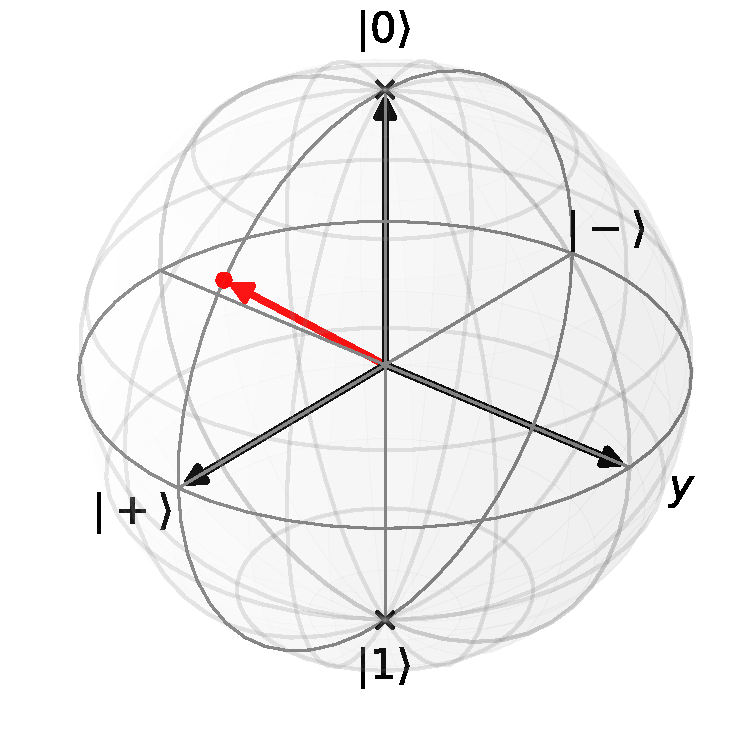
\includegraphics[width=0.7\textwidth]{figures/blochsphere.pdf}
\caption{Darstellung von Quantenbits innerhalb der Bloch-Kugel}
\end{figure}
Da die Bloch-Kugel ein Unterraum des Hilbertraums ist und jede Linearkombination zul\"assiger Vektoren innerhalb dieses Unterraums, wieder einen zul\"assigen Vektor bilden, gibt es unendlich viele Punkte auf der Bloch-Kugel.


\section{Multiple Quantenbits und Quantenregister}
Um Algorithmen oder aufwendige Berechnungen auf Quantencomputern auszuf\"uhren wird mehr als nur ein Qubit bzw. ein Bit an Information ben\"ontigt. Daher ist es wichtig zu verstehen, wie einzelne Qubits miteinander Interagieren, sich zusammenf\"ugen lassen und durch Vektoren beschrieben werden. \\

Das Kronecker-Produkt wird genutzt um Qubits Zusammenzuf\"uhren, bzw. deren kollektiven Zustand zu bilden. \ref{kollektiver-Zustand} zeigt zwei m\"ogliche kollektive Zust\"ande der Basiszust\"ande aus \ref{first}.
\begin{equation}\label{kollektiver-Zustand}
\begin{aligned}
  |0\rangle\otimes |1\rangle = |01\rangle = \begin{bmatrix}1 \times \begin{bmatrix} 0\\1\end{bmatrix}\\[1em] 0 \times \begin{bmatrix} 0\\1\end{bmatrix}\end{bmatrix} = \begin{bmatrix} 0 \\ 1 \\ 0 \\ 0\end{bmatrix} \\[1em]
  |0\rangle\otimes |0\rangle = |00\rangle = \begin{bmatrix}1 \times \begin{bmatrix} 1\\0\end{bmatrix}\\[1em] 0 \times \begin{bmatrix} 1\\0\end{bmatrix}\end{bmatrix} = \begin{bmatrix} 1 \\ 0 \\ 0 \\ 0\end{bmatrix}
\end{aligned}
\end{equation}
Somit lassen sich alle vier Basiszust\"ande, von zwei Qubits aus den zwei Basiszust\"anden von einem Qubit durch das Kronecker-Produkt bilden.
Man gehe davon aus, dass Zust\"ande von mehreren Qubits sich also genau wie Zust\"ande von einzelnen Qubits beschreiben lassen. $n$ Qubits besitzen $2^n$ Amplituden, d.h. diese wachsen exponentiell mit der genutzten Anzahl an Qubits.
\begin{equation}\label{two-qubits}
|\psi \rangle = \alpha_{00} |00\rangle + \alpha_{01} |01\rangle + \alpha_{10} |10\rangle + \alpha_{11} |11\rangle = \begin{bmatrix} \alpha_{00} \\ \alpha_{01} \\ \alpha_{10} \\ \alpha_{11} \end{bmatrix}
\end{equation}
Eine allgemeine Darstellung eines Zustands von zwei Qubits zeigt \ref{two-qubits}, ein 4-Dimensionaler Vektor mit den jeweiligen Amplituden. Auch das quadrieren dieser Ampltiuden zeigt, mit welcher Wahrscheinlichkeit eines der 4 Ergebnisse 00, 01, 10, 11 nach der Messung dieses Zustands erhalten wird.
Das hei\ss t auch dieser Zustand muss durch seine Ampltiuden normalisiert sein, also muss z.B. f\"ur den Zustandsvektor aus \ref{two-qubits} gelten
\begin{equation}
|\alpha_{00}|^2+|\alpha_{01}|^2+|\alpha_{10}|^2+|\alpha_{11}|^2 = 1 .
\end{equation}
Ebenso werden diese Zust\"ande wie in \ref{messung} dargestellt gemessen um z.B. die Wahrscheinlichkeit zu erfahren, das sich der Zustand $|\psi \rangle$ in Zustand $|11\rangle$ befindet wird folgende Messung durchgef\"uhrt.
\begin{equation}
p(|11\rangle) = |\langle 11| \psi  \rangle|^2 = |\alpha_{11}|^2
\end{equation}
Ebenso k\"onnen auch Messungen, nach den Basisvektoren $|0 \rangle$ und $| 1\rangle$ durchgef\"uhrt werden.
\\
Oft werden Zusammensetzungen aus einzelnen Qubits auch Quantenregister genannt, eine allgemeine und kompakte Form dieser Quantenregister aus \cite{Homeister-2022}, sieht folgenderma\ss en aus
\begin{equation}
R = \sum\limits_{i=0}^{2^{n}-1} \alpha_i |i\rangle
\end{equation}
Somit entspricht $|0\rangle, |1\rangle, \dots, |2^{n}-1\rangle$ den Zust\"anden $|0\dots 0\rangle, |0\dots 1\rangle, \dots, |1\dots 1\rangle$.


\section{Quantengatter}
Um Informationen bzw. Bits zu manipulieren werden Schaltungen ben\"otigt welche Gatter beinhalten, dies gilt f\"ur klassische Rechner und Quantencomputer. Um in der Digitaltechnik die Funktionsweise von Gattern darzustellen werden gerne Wahrheitstabellen genutzt (rechte Spalte Tabelle \ref{table:Qubit-Gatter}). Bekannte Gatter-Typen aus der Digitaltechnik, wie der Negation oder dem Exklusiv-ODER k\"onnen auch in der Welt der Quantencomputer abgebildet werden. Jedoch ist der Aufbau dieser Gatter etwas gew\"ohnungsbed\"urfdig, denn die Realisierung eines auf $n$ Qubits operierenden Gatters erfolgt durch eine unit\"are $2^{n}\times 2^{n}$-Matrix. Die Anwendung eines Gatters auf einen Zustandvektor entspricht mathematisch also einer unit\"aren Transformation auf den Zustandsvektor und f\"uhrt eine Rotation auf der Bloch-Kugel aus. Dies geschieht durch die Bildung des Skalarprodukts \"uber der unit\"aren Matrix und dem Zustandvektor. \\ \\
Eine Matrix wird als unit\"ar bezeichnet, wenn das Produkt aus dieser Matrix und dessen adjungierte Matrix eine Einheitsmatrix bildet.
\begin{equation}
  I = A^{\dagger} A
\end{equation}
Die Adjungierte Matrix wird gebildet, indem alle Eintr\"age in dieser Matrix komplex konjungiert und transponiert werden.
\begin{equation}
  A^{\dagger} = A^{*T}
\end{equation}

Somit sind alle Quantengatter unit\"are Matrizen, genau wie die drei aus der Quantenmechnik bekannten Paulimatrizen $X, Y$ und $Z$ Tabelle \ref{table:Qubit-Gatter}. Diese f\"uhren eine Rotation von $\pi$ um die $x, y$ und $z$-Achse auf der Bloch-Kugel durch. Das Hadamard-Gatter $H$ erm\"oglicht eine Abweichung der Basiszust\"ande $|0\rangle$ und $|1\rangle$ und erlaubt eine Superposition dieser Zust\"ande \cite{Qiskit-Textbook}.
Dies w\"aren die Zustandvektoren $|+\rangle$ und $|-\rangle$, welche auch auf der Bloch-Kugel in Abbildung \ref{fig:Bloch-Kugel} zu erkennen sind. \\ \\
Zwei parametrisierte Gatter, das $P$-Gatter (Phasen-Gatter) und $U$-Gatter die nicht in Tabelle \ref{table:Qubit-Gatter} aufgef\"uhrt sind, erlauben die Spezifizierung von s\"amtlichen Gattern bzw. unedlich vielen Gattern.
\begin{equation}
\begin{aligned}
P(\phi) &= \begin{bmatrix}1 & 0 \\ 0 & e^{i\phi} \end{bmatrix} &&\qquad \phi \in \mathbf{R}\\[1em]
U(\theta, \phi, \lambda) &= \begin{bmatrix} \cos\left(\frac{\theta}{2}\right) & -e^{i\lambda}sin\left(\frac{\theta}{2}\right) \\
e^{i\phi}sin\left(\frac{\theta}{2}\right) & e^{i(\phi+\lambda)}sin\left(\frac{\theta}{2}\right)
\end{bmatrix} &&\qquad \theta, \phi, \lambda \in \mathbf{R}
\end{aligned}
\end{equation}

\vspace{1.2cm}
%%%%%%%%%%%%%%%%%%%%%%%Table%%%%%%%%%%%%%%%%%%%%%%%%%%%%%%%%

\begin{table}[h] 
\begin{tabular}{@{\hspace{0.7cm}}c@{\hspace{0.7cm}} | @{\hspace{0.7cm}}c@{\hspace{0.7cm}} | @{\hspace{0.8cm}}c@{\hspace{0.7cm}}}
\hline 
Matrix & Schaltungssymbol & Wahrheitstabelle \\
\hline & \\
$X = \begin{bmatrix} 0 & 1 \\ 1 & 0 \end{bmatrix}$ &
\raisebox{-.3\height}{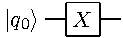
\includegraphics[width=0.2\textwidth]{figures/pauli_x.pdf}} &
\begin{tabular}{|c||c||c|}
\hline
Fall & $|q\rangle$ & $X|q\rangle$ \\
\hline \hline 
1 & $|0\rangle$ & $|1\rangle$ \\
2 & $|1\rangle$ & $|0\rangle$ \\
\hline
\end{tabular} \\&\\

%%%%%%%%%%%%%%%%%%%%%%%%%%%%%%%%%%%%%%%%%%%%%%%%%%%%%%%%%%%%%%

$Y = \begin{bmatrix} 0 & -i \\ i & 0 \end{bmatrix}$ &
\raisebox{-.3\height}{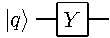
\includegraphics[width=0.2\textwidth]{figures/pauli_y.pdf}} &
\begin{tabular}{|c||c||c|}
\hline
Fall & $|q\rangle$ & $Y|q\rangle$ \\
\hline \hline 
1 & $|0\rangle$ & $i|1\rangle$ \\
2 & $|1\rangle$ & $-i|0\rangle$ \\
\hline
\end{tabular} \\&\\

%%%%%%%%%%%%%%%%%%%%%%%%%%%%%%%%%%%%%%%%%%%%%%%%%%%%%%%%%%%%%%

$Z = \begin{bmatrix} 1 & 0 \\ 0 & -1 \end{bmatrix}$ &
\raisebox{-.3\height}{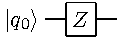
\includegraphics[width=0.2\textwidth]{figures/pauli_z.pdf}} &
\begin{tabular}{|c||c||c|}
\hline
Fall & $|q\rangle$ & $Z|q\rangle$ \\
\hline \hline 
1 & $|0\rangle$ & $|0\rangle$ \\
2 & $|1\rangle$ & $-|1\rangle$ \\
\hline
\end{tabular} \\&\\

%%%%%%%%%%%%%%%%%%%%%%%%%%%%%%%%%%%%%%%%%%%%%%%%%%%%%%%%%%%%%%

$H = \frac{1}{\sqrt{2}} \begin{bmatrix} 1 & 1 \\ 1 & -1 \end{bmatrix}$ &
\raisebox{-.3\height}{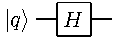
\includegraphics[width=0.2\textwidth]{figures/hadamard.pdf}} &
\begin{tabular}{|c||c||c|}
\hline
Fall & $|q\rangle$ & $H|q\rangle$ \\
\hline \hline 
1 & $|0\rangle$ & $\frac{|0\rangle+|0\rangle}{\sqrt{2}}$ \\
2 & $|1\rangle$ & $\frac{|0\rangle-|1\rangle}{\sqrt{2}}$ \\
\hline
\end{tabular} \\&\\

%%%%%%%%%%%%%%%%%%%%%%%%%%%%%%%%%%%%%%%%%%%%%%%%%%%%%%%%%%%%%%

$S = \begin{bmatrix} 1 & 0 \\ 0 & i \end{bmatrix}$ &
\raisebox{-.3\height}{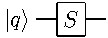
\includegraphics[width=0.2\textwidth]{figures/phase.pdf}} &
\begin{tabular}{|c||c||c|}
\hline
Fall & $|q\rangle$ & $S|q\rangle$ \\
\hline \hline 
1 & $|0\rangle$ & $|0\rangle$ \\
2 & $|1\rangle$ & $i|1\rangle$ \\
\hline
\end{tabular} \\&\\

%%%%%%%%%%%%%%%%%%%%%%%%%%%%%%%%%%%%%%%%%%%%%%%%%%%%%%%%%%%%%%

$T = \begin{bmatrix} 1 & 0 \\ 0 & e^{i\frac{\pi}{4}} \end{bmatrix}$ &
\raisebox{-.3\height}{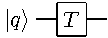
\includegraphics[width=0.2\textwidth]{figures/t_dagger.pdf}} &
\begin{tabular}{|c||c||c|}
\hline
Fall & $|q\rangle$ & $T|q\rangle$ \\
\hline \hline 
1 & $|0\rangle$ & $|0\rangle$ \\
2 & $|1\rangle$ & $e^{i\frac{\pi}{4}} |1\rangle$ \\
\hline
\end{tabular} \\&\\
\hline
\end{tabular}
\caption{Grundlegende 1-Qubit Gatter}
\label{table:Qubit-Gatter}
\end{table}
\clearpage

Aus dem $P$-Gatter lassen sich die Gatter $Z, S$ und $T$ konstruieren. \ref{eqn:konstruktion} zeigt die Spezifizierung der $S$- und $T$-Gatter durch das Phasengatter.
\begin{equation}\label{eqn:konstruktion}
P\left(\phi=\frac{\pi}{2}\right) = S \qquad P(\phi=\pi) = Z .
\end{equation}

Das $U$-Gatter erm\"oglicht die Spezifizierung jeglicher Gatter, z.B. kann das Hadamard-Gatter folgenderma\ss en durch das $U$-Gatter spezifiziert werden
\begin{equation}
U\left(\theta= \frac{\pi}{2}, \phi=0, \lambda=\pi\right) = H .
\end{equation}
Somit kann es eine gro\ss e Menge an n\"utzlichen Gattern geben, die auf einem Qubit operieren. Jedoch ist es m\"oglich diese Gatter auch auf meheren Qubits operieren zu lassen. Diese Gatter werden dann kontrollierte Gatte gennant, da diese ein oder mehrere kontrollierende \textit{(control)} Qubits und ein Ziel Qubit \textit{(target)} beinhalten. Tabelle \ref{table:2Qubit-Gatter} zeigt oft genutzte Gatter die auf mehr als einem Qubit operieren.
%%%%%%%%%%%%%%%%%%%%%%%Table Multi%%%%%%%%%%%%%%%%%%%%%%%%%%%%%%%%

\begin{table}[h]
\hspace{-1cm}
\begin{tabular}{c|c|c}
\hline 
Matrix & Schaltungssymbol & Wahrheitstabelle \\
\hline & \\
$CX_{01} = \begin{bmatrix} 1 & 0 & 0 & 0 \\ 0 & 1 & 0 & 0 \\ 0 & 0 & 0 & 1 \\ 0 & 0 & 1 & 0 \end{bmatrix}$ &
\raisebox{-.5\height}{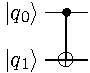
\includegraphics[width=0.16\textwidth]{figures/cnot.pdf}} &
\begin{tabular}{|c||c||c|}
\hline
Fall & $|q_0 q_1\rangle$ & $CX_{01}|q_0 q_1\rangle$ \\
\hline \hline 
1 & $|00\rangle$ & $|00\rangle$ \\
2 & $|01\rangle$ & $|01\rangle$ \\
3 & $|10\rangle$ & $|11\rangle$ \\
4 & $|11\rangle$ & $|10\rangle$ \\
\hline
\end{tabular} \\&\\

%%%%%%%%%%%%%%%%%%%%%%%%%%%%%%%%%%%%%%%%%%%%%%%%%%%%%%%%%%%%%%

$CZ_{01} = \begin{bmatrix} 1 & 0 & 0 & 0 \\ 0 & 1 & 0 & 0 \\ 0 & 0 & 1 & 0 \\ 0 & 0 & 0 & -1 \end{bmatrix}$ &
\raisebox{-.5\height}{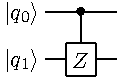
\includegraphics[width=0.2\textwidth]{figures/cz.pdf}} &
\begin{tabular}{|c||c||c|}
\hline
Fall & $|q_0 q_1\rangle$ & $CZ_{01}|q_0 q_1\rangle$ \\
\hline \hline 
1 & $|00\rangle$ & $|00\rangle$ \\
2 & $|01\rangle$ & $|01\rangle$ \\
3 & $|10\rangle$ & $|10\rangle$ \\
4 & $|11\rangle$ & $-|11\rangle$ \\
\hline
\end{tabular} \\&\\

%%%%%%%%%%%%%%%%%%%%%%%%%%%%%%%%%%%%%%%%%%%%%%%%%%%%%%%%%%%%%%

$SWAP = \begin{bmatrix} 1 & 0 & 0 & 0 \\ 0 & 0 & 1 & 0 \\ 0 & 1 & 0 & 0 \\ 0 & 0 & 0 & 1 \end{bmatrix}$ &
\raisebox{-.5\height}{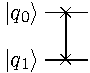
\includegraphics[width=0.16\textwidth]{figures/swap.pdf}} &
\begin{tabular}{|c||c||c|}
\hline
Fall & $|q_0 q_1\rangle$ & $SWAP|q_0 q_1\rangle$ \\
\hline \hline 
1 & $|00\rangle$ & $|00\rangle$ \\
2 & $|01\rangle$ & $|10\rangle$ \\
3 & $|10\rangle$ & $|01\rangle$ \\
4 & $|11\rangle$ & $|11\rangle$ \\
\hline
\end{tabular} \\&\\

%%%%%%%%%%%%%%%%%%%%%%%%%%%%%%%%%%%%%%%%%%%%%%%%%%%%%%%%%%%%%%

$CCX_{012} = \begin{bmatrix} I_2 & 0_2 & 0_2 & 0_2 \\ 0_2 & I_2 & 0_2 & 0_2 \\ 0_2 & 0_2 & I_2 & 0_2 \\ 0_2 & 0_2 & 0_2 & X \end{bmatrix}$ &
\raisebox{-.5\height}{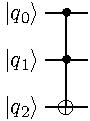
\includegraphics[width=0.16\textwidth]{figures/toffoli.pdf}} &
\begin{tabular}{|c||c||c|}
\hline
Fall & $|q_0 q_1 q_2 \rangle$ & $CCX_{012}|q_0 q_1 q_2\rangle$ \\
\hline \hline 
1 & $|000\rangle$ & $|000\rangle$ \\
2 & $|001\rangle$ & $|001\rangle$ \\
3 & $|010\rangle$ & $|010\rangle$ \\
4 & $|011\rangle$ & $|011\rangle$ \\
5 & $|100\rangle$ & $|100\rangle$ \\
6 & $|101\rangle$ & $|101\rangle$ \\
7 & $|110\rangle$ & $|111\rangle$ \\
8 & $|111\rangle$ & $|110\rangle$ \\
\hline
\end{tabular} \\&\\

%%%%%%%%%%%%%%%%%%%%%%%%%%%%%%%%%%%%%%%%%%%%%%%%%%%%%%%%%%%%%%

$CS_{10} = \begin{bmatrix} 1 & 0 & 0 & 0 \\ 0 & 0 & 0 & e^{i\phi} \\ 0 & 1 & 0 & 0 \\ 0 & 0 & 1 & 0 \end{bmatrix}$ &
\raisebox{-.5\height}{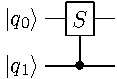
\includegraphics[width=0.2\textwidth]{figures/cs.pdf}} &
\begin{tabular}{|c||c||c|}
\hline
Fall & $|q_0 q_1\rangle$ & $CS_{10}|q_0 q_1\rangle$ \\
\hline \hline 
1 & $|00\rangle$ & $|00\rangle$ \\
2 & $|01\rangle$ & $|01\rangle$ \\
3 & $|10\rangle$ & $|10\rangle$ \\
4 & $|11\rangle$ & $i|11\rangle$ \\
\hline
\end{tabular} \\&\\
\hline
\end{tabular}
\caption{Ausgew\"ahlte 2-, 3-Quanten Gatter}
\label{table:2Qubit-Gatter}
\end{table}


\section{Quantenschaltungen}



%%%%%%%%%%%%%%%%%%%%%%%%%%%%%%%%%%%%%%%%%%%%%%%%%%%%%%%%%%%%%%%%%%%%%%%%%%%%%%%%
%%%%%%%%%%%%%%%%%%%%%%%%%%%%%%%%%%%%%%%%%%%%%%%%%%%%%%%%%%%%%%%%%%%%%%%%%%%%%%%%
%%%%%%%%%%%%%%%%%%%%%%%%%%%%%%%%%%%%%%%%%%%%%%%%%%%%%%%%%%%%%%%%%%%%%%%%%%%%%%%%
\chapter{Programmierung von Quantencomputer}
\lipsum[1-4]
\section{Software und Programmiersprachen}
\lipsum[1-4]

\section{Simualtion}
Da die Anzahl an komplexen Amplituden exponentiell mit der Nutzung von Quantenbits steigt, ist die Simulation von Quantencomputern nur effizient mit einer Anzahl von $\approx$ 20 Qubits m\"oglich. Selbst die Simulation von Quantencomputern mit 100 Qubits ist auf sehr leistungsf\"ahigen Supercomputer momentan nicht m\"oglich \cite{Qiskit-Textbook}.


\section{Verf�gbare Hardware}
\lipsum[1-4]

%%%%%%%%%%%%%%%%%%%%%%%%%%%%%%%%%%%%%%%%%%%%%%%%%%%%%%%%%%%%%%%%%%%%%%%%%%%%%%%%
%%%%%%%%%%%%%%%%%%%%%%%%%%%%%%%%%%%%%%%%%%%%%%%%%%%%%%%%%%%%%%%%%%%%%%%%%%%%%%%%
%%%%%%%%%%%%%%%%%%%%%%%%%%%%%%%%%%%%%%%%%%%%%%%%%%%%%%%%%%%%%%%%%%%%%%%%%%%%%%%%

\chapter{Implementierung von Quantenalgorithmen}

\lipsum[1-4]

\section{Algorithmen�berblick}
\lipsum[1-4]



%%%%%%%%%%%%%%%%%%%%%%%%%%%%%%%%%%%%%%%%%%%%%%%%%%%%%%%%%%%%%%%%%%%%%%%%%%%%%%%%
%%%%%%%%%%%%%%%%%%%%%%%%%%%%%%%%%%%%%%%%%%%%%%%%%%%%%%%%%%%%%%%%%%%%%%%%%%%%%%%%
%%%%%%%%%%%%%%%%%%%%%%%%%%%%%%%%%%%%%%%%%%%%%%%%%%%%%%%%%%%%%%%%%%%%%%%%%%%%%%%%

\section{Shors Algorithmus}
\label{methods}

\lipsum[1-10]

%%%%%%%%%%%%%%%%%%%%%%%%%%%%%%%%%%%%%%%%%%%%%%%%%%%%%%%%%%%%%%%%%%%%%%%%%%%%%%%%
%%%%%%%%%%%%%%%%%%%%%%%%%%%%%%%%%%%%%%%%%%%%%%%%%%%%%%%%%%%%%%%%%%%%%%%%%%%%%%%%

\section{Umsetzung}
\label{algorithms}

\section{Ergebnisse}
\lipsum[1-10]



%%%%%%%%%%%%%%%%%%%%%%%%%%%%%%%%%%%%%%%%%%%%%%%%%%%%%%%%%%%%%%%%%%%%%%%%%%%%%%%%
%%%%%%%%%%%%%%%%%%%%%%%%%%%%%%%%%%%%%%%%%%%%%%%%%%%%%%%%%%%%%%%%%%%%%%%%%%%%%%%%
%%%%%%%%%%%%%%%%%%%%%%%%%%%%%%%%%%%%%%%%%%%%%%%%%%%%%%%%%%%%%%%%%%%%%%%%%%%%%%%%



%%%%%%%%%%%%%%%%%%%%%%%%%%%%%%%%%%%%%%%%%%%%%%%%%%%%%%%%%%%%%%%%%%%%%%%%%%%%%%%%
%%%%%%%%%%%%%%%%%%%%%%%%%%%%%%%%%%%%%%%%%%%%%%%%%%%%%%%%%%%%%%%%%%%%%%%%%%%%%%%%
%%%%%%%%%%%%%%%%%%%%%%%%%%%%%%%%%%%%%%%%%%%%%%%%%%%%%%%%%%%%%%%%%%%%%%%%%%%%%%%%

\chapter{Fazit}
\label{conclusions}

\lipsum[1-10]

%%%%%%%%%%%%%%%%%%%%%%%%%%%%%%%%%%%%%%%%%%%%%%%%%%%%%%%%%%%%%%%%%%%%%%%%%%%%%%%%
%%%%%%%%%%%%%%%%%%%%%%%%%%%%%%%%%%%%%%%%%%%%%%%%%%%%%%%%%%%%%%%%%%%%%%%%%%%%%%%%

\section{Zuk�nftige Arbeiten}

\lipsum[1-10]

%%%%%%%%%%%%%%%%%%%%%%%%%%%%%%%%%%%%%%%%%%%%%%%%%%%%%%%%%%%%%%%%%%%%%%%%%%%%%%%%
%%%%%%%%%%%%%%%%%%%%%%%%%%%%%%%%%%%%%%%%%%%%%%%%%%%%%%%%%%%%%%%%%%%%%%%%%%%%%%%%

\section{Zusammenfassung}

\lipsum[1-10]

%%%%%%%%%%%%%%%%%%%%%%%%%%%%%%%%%%%%%%%%%%%%%%%%%%%%%%%%%%%%%%%%%%%%%%%%%%%%%%%%
%%%%%%%%%%%%%%%%%%%%%%%%%%%%%%%%%%%%%%%%%%%%%%%%%%%%%%%%%%%%%%%%%%%%%%%%%%%%%%%%
%%%%%%%%%%%%%%%%%%%%%%%%%%%%%%%%%%%%%%%%%%%%%%%%%%%%%%%%%%%%%%%%%%%%%%%%%%%%%%%% 
%%%%%%%%%%%%%%%%%%%%%%%%%%%%%%%%%%%%%%%%%%%%%%%%%%%%%%%%%%%%%%%%%%%%%%%%%%%%%%%%
%%%%%%%%%%%%%%%%%%%%%%%%%%%%%%%%%%%%%%%%%%%%%%%%%%%%%%%%%%%%%%%%%%%%%%%%%%%%%%%%
%%%%%%%%%%%%%%%%%%%%%%%%%%%%%%%%%%%%%%%%%%%%%%%%%%%%%%%%%%%%%%%%%%%%%%%%%%%%%%%%

%%%
%%% end main document
%%%
%%%%%%%%%%%%%%%%%%%%%%%%%%%%%%%%%%%%%%%%%%%%%%%%%%%%%%%%%%%%%%%%%%%%%%%%%%%%%%%%

\appendix  %% include it, if something (bibliography, index, ...) follows below


\chapter{Anhang}

\lipsum[2]


%\afterpage{\blankpage}
%%%%%%%%%%%%%%%%%%%%%%%%%%%%%%%%%%%%%%%%%%%%%%%%%%%%%%%%%%%%%%%%%%%%%%%%%%%%%%%%
%%%%%%%%%%%%%%%%%%%%%%%%%%%%%%%%%%%%%%%%%%%%%%%%%%%%%%%%%%%%%%%%%%%%%%%%%%%%%%%%
%%%%%%%%%%%%%%%%%%%%%%%%%%%%%%%%%%%%%%%%%%%%%%%%%%%%%%%%%%%%%%%%%%%%%%%%%%%%%%%%
%%%%%%%%%%%%%%%%%%%%%%%%%%%%%%%%%%%%%%%%%%%%%%%%%%%%%%%%%%%%%%%%%%%%%%%%%%%%%%%%
%%%%%%%%%%%%%%%%%%%%%%%%%%%%%%%%%%%%%%%%%%%%%%%%%%%%%%%%%%%%%%%%%%%%%%%%%%%%%%%%
%%%%%%%%%%%%%%%%%%%%%%%%%%%%%%%%%%%%%%%%%%%%%%%%%%%%%%%%%%%%%%%%%%%%%%%%%%%%%%%%

%%%%%%%%%%%%%%%%%%%%%%%%%%%%%%%%%%%%%%%%%%%%%%%%%%%%%%%%%%%%%%%%%%%%%%%%%%%%%%%%
%%%
%%% bibliography
%%%
%%% available styles: abbrv, acm, alpha, apalike, ieeetr, plain, siam, unsrt
%%%
\bibliographystyle{ieeetr}

%%% name of the bibliography file without .bib
%%% e.g.: literatur.bib -> \bibliography{literatur}
\bibliography{literature.bib}

\end{document}
%%% }}}
%%% END OF FILE
%%%%%%%%%%%%%%%%%%%%%%%%%%%%%%%%%%%%%%%%%%%%%%%%%%%%%%%%%%%%%%%%%%%%%%%%%%%%%%%%
%%% Notice!
%%% This file uses the outline-mode of emacs and the foldmethod of Vim.
%%% Press 'zi' to unfold the file in Vim.
%%% See ':help folding' for more information.
%%%%%%%%%%%%%%%%%%%%%%%%%%%%%%%%%%%%%%%%%%%%%%%%%%%%%%%%%%%%%%%%%%%%%%%%%%%%%%%%
%% Local Variables:
%% mode: outline-minor
%% OPToutline-regexp: "%% .*"
%% OPTeval: (hide-body)
%% emerge-set-combine-versions-template: "%a\n%b\n"
%% End:
%% vim:foldmethod=marker
